%\documentclass[handout]{beamer}
\documentclass{beamer}

\usepackage{color}
\usepackage{beamerthemesplit}
\usepackage[utf8]{inputenc}

%\usetheme{Malmoe}
%\usetheme{CambridgeUS}
%\usetheme{Hannover}

% Tema Simple
\usetheme[height=0.35cm]{Madrid}

% El que uso habitualmente:
%\usetheme[height=0.7cm]{Rochester}

% A dark look
%\usecolortheme{beetle}
\usecolortheme{dolphin}

\setbeamertemplate{navigation symbols}{} 

%\usepackage{wrapfig}
\setbeamercovered{transparent}

\usepackage{geometry}
%\geometry{landscape}
\usepackage{multimedia}
\usepackage{verbatim}
\usepackage{bm}%bold matH

%\usepackage{shade}
\usepackage{fancybox}
 
\usepackage{amssymb}

\input{Definiciones.coloquio}
%\input{Definiciones.charla}


\vspace*{-0.75 cm}
\title[Corona Solar 3D]{\bf Estudio tomográfico de validación para el modelo MHD AWSoM en la baja corona solar}
\author[D. Lloveras]
       {{\bf Diego G. Lloveras}\inst{1}\\
       \vskip 0.1cm
       {
        C. Mac Cormack\inst{1}, A.M. Vásquez \inst{1}, F.A. Nuevo\inst{1}, N. Sachdeva\inst{2}, W. Manchester IV\inst{2}, B. Van der Holst\inst{2} y R.A. Frazin\inst{2}
       }
      % \\
       }
  \institute[IAFE]
  {
  \inst{1}
%  Institute for Astronomy and Space Physics \textcolor{blue}{(IAFE)} \\ 
  Instituto de Astronom\'{\i}a y F\'{\i}sica del Espacio \textcolor{blue}{(IAFE)} \\ 
  CONICET-UBA, Ciudad de Buenos Aires, Argentina
  \and
  \inst{2}
%  Dept. of Atmospheric, Oceanic and Space Sciences \textcolor{blue}{(AOSS)}\\
  Dept. of Climate and Space Sciences and Engineering \textcolor{blue}{(CLaSP)}\\
  University of Michigan, Ann Arbor - Michigan, USA
  \salto
%  \vspace{-0.25cm}
  \begin{center}
\framebox{\includegraphics[height=0.15\linewidth]{new_figs/logo_IAFE.eps}}
%\framebox{\includegraphics[height=0.1\linewidth]{logo_LMSAL.eps}}
\framebox{\includegraphics[height=0.15\linewidth]{new_figs/logo_clasp2.eps}}
\framebox{\includegraphics[height=0.15\linewidth]{new_figs/aaa_logo.png}}
\salto
{\bf AAA \textbar \ Septiembre-2019 \textbar \ Viedma, Argentina}
\end{center}
  }

\begin{document}

%Pagina Inicial
\frame{\titlepage}

%-------------------> INTRODUCCION <----------------------------------------------------

\frame{
\titulo{Solar Corona and Sun-Earth relation}
\scriptsize
\framebox{\includegraphics[width=\linewidth]{new_figs/Sun-Earth.eps}}
\begin{center}
%La observación y el modelado de la Corona solar resulta de gran relevancia para el entendimiento de la relación Sol-Tierra, ya que en la Corona es donde el viento solar es calentado, acelerado y tienen lugar eventos impulsivos como eyecciones de masa coronal, flares, etc.

Being the place where the solar wind is heated and accelerated, and impulsive events as solar flares and coronal mass ejections are released, observation and modeling of the Solar Corona is of great relevance to advance our understanding of the Sun-Earth environment.
%Advancement of physical models is in need of 3D information of the coronal fundamental parameters ${\bf B}, N_e, T_e$ and chemical abundances.
\end{center}
}

%-------------------------------------------------------------------
\begin{comment}
\frame{
\titulo{Solar Structure}
\scriptsize
\begin{columns}
\column{0.5\textwidth}
%\ \hskip 1cm \azul{Interior}
%\begin{itemize}
%\item Core (T$\approx 15$\, MK)
%\item Radiative Z. (T$\approx 10-0.5$\, MK)
%\item Convective Z. (T$\approx 0.5\,{\rm MK} - 6.5$\, kK)
%\end{itemize}
\vspace{0.55cm}
\begin{center}
{\includegraphics[width=0.9\textwidth]{new_figs/SolarStructure.eps}}
\end{center}
\column{0.55\textwidth}
\ \hskip 1cm \azul{Atmosphere}
\begin{itemize}
\item Photosphere (T $\approx 5.5$\, kK, $n \approx 10^{17}\ {\rm cm}^{-3}$)
\item Chromosphere (T $\approx 20$\, kK, $n \approx 10^{11}\ {\rm cm}^{-3}$)
\item Transition Region (Thickness 100 km)
\item Corona (T $\approx 1-10$\, MK, $n \approx 10^{10-7}\ {\rm cm}^{-3}$)
\end{itemize}
\begin{center}
{\includegraphics[width=0.675\textheight]{new_figs/region_transicion_fede.eps}}
\end{center}
\end{columns}
}
\end{comment}
%---------------------------------------------------------------------------
\frame{
\titulo{Solar Corona}
\footnotesize
\vspace{-0.25cm}
\begin{center}
{\includegraphics[width=0.35\textwidth]{new_figs/SolarStructure.eps}}
{\includegraphics[width=0.5\textwidth]{new_figs/region_transicion_fede.eps}}
\end{center}
 Corona (T $\approx 1-10$\, MK, $n \approx 10^{10-7}\ {\rm cm}^{-3}$)
\begin{itemize}
 %\item La baja corona emite eficientemente en el rango EUV.\\
 \item The corona is \azul{optically thin} in the UV, \azul{EUV}, X, \azul{WL} ranges.\\
%Las imágenes son proyecciones 2D de estructuras emisoras 3D.
\item Images are thus 2D projections of the underlying 3D emitting structure.
% \salto
% \item El plasma emisor es governado por el \azul{campo magn\'etico coronal} congelado a la materia, para el cual {no se dispone de mediciones} (que son fotosf\'ericas).
 \mediosalto
%\item Los modelos físicos necesitan información 3D coronal de parámetros $N_e, T_e$.
\item Advancement of physical models is in need of 3D information of the coronal fundamental parameters ${\bf B}, N_e, T_e$ and chemical abundances.
\end{itemize}
%\vspace{0.35cm}
%\azul{\bf Tomography}\\
%\vspace{0.15cm}
%By inverting for the \azul{3D EUV emissivity from time series of images} it allows inferring the 3D $N_e$ and $T_e$ of the global corona.
%\begin{columns}
%\column{0.5\textwidth}
%\begin{center}
%AIA \\
%{\includegraphics[height=0.3\textwidth]{new_figs/2017_12_15_19_11_15_AIA_171.png}}
%{\includegraphics[height=0.3\textwidth]{new_figs/2017_12_15_19_11_15_AIA_193.png}}
%{\includegraphics[height=0.3\textwidth]{new_figs/2017_12_15_19_11_15_AIA_211.png}}
%\azul{\bf Stereoscopy}
%{\includegraphics[height=0.65\textwidth]{figuras/aia_171_loops.eps}}
%\\
%By studying the \azul{2D shape of EUV loops from 2 view points} it infers the 3D geometry of their "frozen-in" magnetic loops.
%\end{center}
%\column{0.5\textwidth}
%\begin{center}
%COSMO K-coronograph
%{\includegraphics[height=0.7\textwidth]{new_figs/20171215_175739_kcor_l15_extavg.eps}}
%{\includegraphics[height=0.7\textwidth]{figuras/aia_193_fullsun.eps}}
%Invierte una serie temporal de imágenes EUV permitiendo inferir la distribución 3D de $N_e$ y $T_e$ en la baja corona.\\
%(Frazin et al. 2005)
%By inverting for the \azul{3D EUV emissivity from time series of images} it allows inferring the 3D $N_e$ and $T_e$ of the global corona.
%\end{center}
%\end{columns}

}
%------------------------------
\frame{
\titulo{Tomografía Solar Rotacional (TSR)}
\footnotesize
\vspace{-0.2cm}
\begin{center}
%The corona is \azul{optically thin} in the UV, \azul{EUV}, X, \azul{WL} ranges.\\
%By inverting for the \azul{3D EUV emissivity from time series of images} it allows inferring the 3D $N_e$ and $T_e$ of the global corona.
%The object of study is the solar corona.\\
%The solar rotation provides the necessary 360\deg view angles.
El objeto de estudio es la Corona Solar.\\
La rotación solar provee los diferentes ángulos de visión necesarios.
\end{center}
%\vspace{-1.5cm}
\begin{columns}
%\vspace{-1cm}
\column{0.6\textwidth}
\begin{itemize}
\item \azul{Corona-E:} Emisión de iones coronales en UV, \azul{EUV} y X.
\item \azul{TSR-EUV} $\rightarrow$ emisividad EUV 3D  $\rightarrow$\\
Medida de Emisión Diferencial 3D $\rightarrow$\\
$N_e$ y $T_e$ 3D
\item 1$^{\rm er}$ TSR-EUV:\\ 
Frazin, Vásquez \& Kamalabadi (ApJ 2009)\\
Vásquez, Frazin \& Kamalabadi (SolPhys 2009)
\end{itemize}
\column{0.4\textwidth}
%\vskip 1.2cm
\begin{center}
%\azul{White Light}
%\includegraphics[height=0.7\textwidth]{new_figs/20171215_175739_kcor_l15_extavg.eps}
%\includegraphics[height=0.6\textwidth]{new_figs/LASCOC2_comet.eps}
\mediosalto
\azul{EUV} \\
\includegraphics[height=0.6\textwidth]{new_figs/2017_12_15_19_11_15_AIA_171.png}
%\includegraphics[height=0.3\textwidth]{new_figs/2017_12_15_19_11_15_AIA_193.png}
%\includegraphics[height=0.3\textwidth]{new_figs/2017_12_15_19_11_15_AIA_211.png}
\end{center}
\end{columns}

\begin{columns}
\column{0.1\textwidth}
\vskip 1cm
195 \AA\\
1.5 MK
\column{0.2\textwidth}
\begin{center}
Long = 360\deg\\
\framebox{\includegraphics[width=\linewidth]
{new_figs/195_360.eps}}
\end{center}
\column{0.2\textwidth}
\begin{center}
Long = 270\deg\\
\framebox{\includegraphics[width=\linewidth]
{new_figs/195_270.eps}}
\end{center}
\column{0.2\textwidth}
\begin{center}
Long = 180\deg\\
\framebox{\includegraphics[width=\linewidth]
{new_figs/195_180.eps}}
\end{center}
\column{0.2\textwidth}
\begin{center}
Long = 90\deg\\
\framebox{\includegraphics[width=\linewidth]
{new_figs/195_90.eps}}
\end{center}
\end{columns}
}

%-----------------------------------
\frame{ 
\vspace{-0.35cm}
\begin{columns}
\noindent
\column{0.075\textwidth}
\vskip 0.8cm
{\footnotesize
\ 171 \AA
\vskip 1.75cm
\ 195 \AA
\vskip 1.65cm
\ 284 \AA
}
\column{\textwidth}
\begin{center}
{\footnotesize
\ \ Data Images \hfill $\rightarrow$ \hfill 3D Band Emissivity \hfill $\rightarrow$ \hfill Synthetic Images\ \ \ \
}\\
\framebox{\includegraphics[width=0.95\linewidth]{new_figs/frame_050_test.pdf}}\\
\footnotesize
 1.035 $\mrsun$ \hskip 1cm 1.085 $\mrsun$ \hskip 1cm 1.135 $\mrsun$ \hfil
\end{center}
\end{columns}
%\begin{columns}
% \column{0.4\textwidth}
 $
\azul{I_{k,j}} = \azul{
\int_{\mathrm{LOS}} \mathrm{d}l} \ 
\rojo{FBE_k \left(\azul{\br_j(l)}\right)}
$  \hfill Vásquez et al. (2016)
% \column{0.6\textwidth}
%\end{columns}
}
%-------------------------------
\frame{
\titulo{Characteristic Temperatures of the Solar Corona}
\footnotesize
\begin{center}
EIT/SOHO and EUVI/STEREO \azul{3 bands:} \azul{0.5-2.75 MK}\\
{AIA/SDO} \azul{4 bands:} \azul{0.5-4.0 MK},\\
\begin{figure}[ht]
\figu{\includegraphics[height=0.375\linewidth]{new_figs/panel.eps}}
\figu{\includegraphics[height=0.375\linewidth]{new_figs/qkl.eps}}
\end{figure}
\end{center}
%\tiny
$\azul{FBE_{k,i} }  =  \azul{\int \mathrm{d}T \  R_k(T)  \rojo{{\sf LDEM}_i(T)} }$ $\rightarrow$
$\left< N_e^2\right>_i = \int \mathrm{d} T \ \, \rojo{{\sf LDEM}_i(T)}$\\
\qquad \qquad \qquad \qquad \qquad \qquad \qquad $\rightarrow$ $T_{m,i}   = \frac{1}{\left< N_e^2\right>_i } \int \mathrm{d}T\ T \ \, \rojo{{\sf LDEM}_i(T)}$\\
}

%---------------------------------
\frame{ 
\vspace{-0.05cm}
\titulo{Example of EUV Tomography}
\footnotesize

\begin{center}
  Minimum 2009 Extreme UltraViolet Imager\\

%{\includegraphics[width=0.86\textwidth]{new_figs/Ne_1105_cr2081l075_ldem_v3_errorbox_base_test.jpg}}
{\includegraphics[width=0.46\textwidth]{new_figs/Ne_1025_CR2081.pdf}}
%{\includegraphics[width=0.86\textwidth]{new_figs/Tm_1105_cr2081l075_ldem_v3_errorbox_base_test.jpg}}\\
{\includegraphics[width=0.46\textwidth]{new_figs/Tm_1025_CR2081.pdf}}\\
%{\includegraphics[width=0.86\textwidth]{new_figs/Ne_1105_cr1915l075_ldem_v3_errorbox_base_test.jpg}}
{\includegraphics[width=0.46\textwidth]{new_figs/Ne_1105_CR2081.pdf}}
%{\includegraphics[width=0.86\textwidth]{new_figs/Tm_1105_cr1915l075_ldem_v3_errorbox_base_test.jpg}}\\
{\includegraphics[width=0.46\textwidth]{new_figs/Tm_1105_CR2081.pdf}}
\end{center}
(Lloveras et al. 2017) $\rightarrow$ Systematic uncertainties in DEMT results $\sim 10 \%$
}
%---------------------------------
\begin{comment}
\frame{
%\titulo{Instruments}
\footnotesize
\begin{columns}
\column{0.33\textwidth}
\begin{center}
Instruments \\
AIA - SDO\\
\includegraphics[height=0.6\textwidth]{new_figs/sdo.eps} \\
\mediosalto
K-Coronograph - COSMO \\
\includegraphics[height=0.9\textwidth]{new_figs/kcor.eps}
\end{center}
\column{0.33\textwidth}
\begin{center}
Images\\
Emission of the Fe lines \\
\includegraphics[height=0.33\textwidth]{new_figs/2017_12_15_19_11_15_AIA_171.png}
\includegraphics[height=0.33\textwidth]{new_figs/2017_12_15_19_11_15_AIA_193.png}
\includegraphics[height=0.33\textwidth]{new_figs/2017_12_15_19_11_15_AIA_211.png}
\mediosalto
\mediosalto
Polarized brightness \\
\includegraphics[height=0.9\textwidth]{new_figs/20171215_175739_kcor_l15_extavg.eps}
\end{center}
\column{0.33\textwidth}
\begin{center}
\vskip -1.6cm
$\rightarrow$ 3D $<{N_{e}}^{2}>$ \\
\vskip 2.cm
$\rightarrow$ 3D $<N_{e}>$
\end{center}
\end{columns}
}
\end{comment}
%----------------------------------
\frame{
%\titulo{DEMT as MHD Validation Tool \azul{\footnotesize (Jin et al. 2012)}}
\footnotesize
%\vspace{-0.25cm}
%\begin{center}
% AWSoM / Space Weather Modeling Framework (Univ. of Michigan)
%2 Temp MHD Model of the Space Weather Modeling Framework (CLASP)
%\vspace{-0.5cm}
\begin{columns}
\column{0.5\textwidth}
\begin{center}
\includegraphics[width=0.75\textwidth]{new_figs/ne_demt_2208_1055.png}
\includegraphics[width=0.75\textwidth]{new_figs/ne_awsom_2208_1055.png}
\includegraphics[width=0.75\textwidth]{new_figs/ne_diff_2208_1055.png}
\end{center}
\column{0.5\textwidth}
\begin{center}
\includegraphics[width=0.75\textwidth]{new_figs/te_demt_2208_1055.png}
\includegraphics[width=0.75\textwidth]{new_figs/te_awsom_2208_1055.png}
\includegraphics[width=0.75\textwidth]{new_figs/te_diff_2208_1055.png}
\end{center}
\end{columns}
%\end{center}
%Inner Ring (1.00 - 1.25 \rsun): Ratio MHD/DEMT.\\
%- Outter Greyscale map ($>$ 1.25 \rsun): MHD Model.\\
%- Color Sphere: $B_r(1\,{\rm R_{\rm SUN}})$.
%\item
%$N_e$ y $T_e$ also validated with spectral analysis (Hinode/EIS, 1.02-1.10 \rsun).
}
%---------------------------------

\frame{ 
%\vspace{-0.05cm}
%\titulo{a}
\footnotesize
\begin{center}
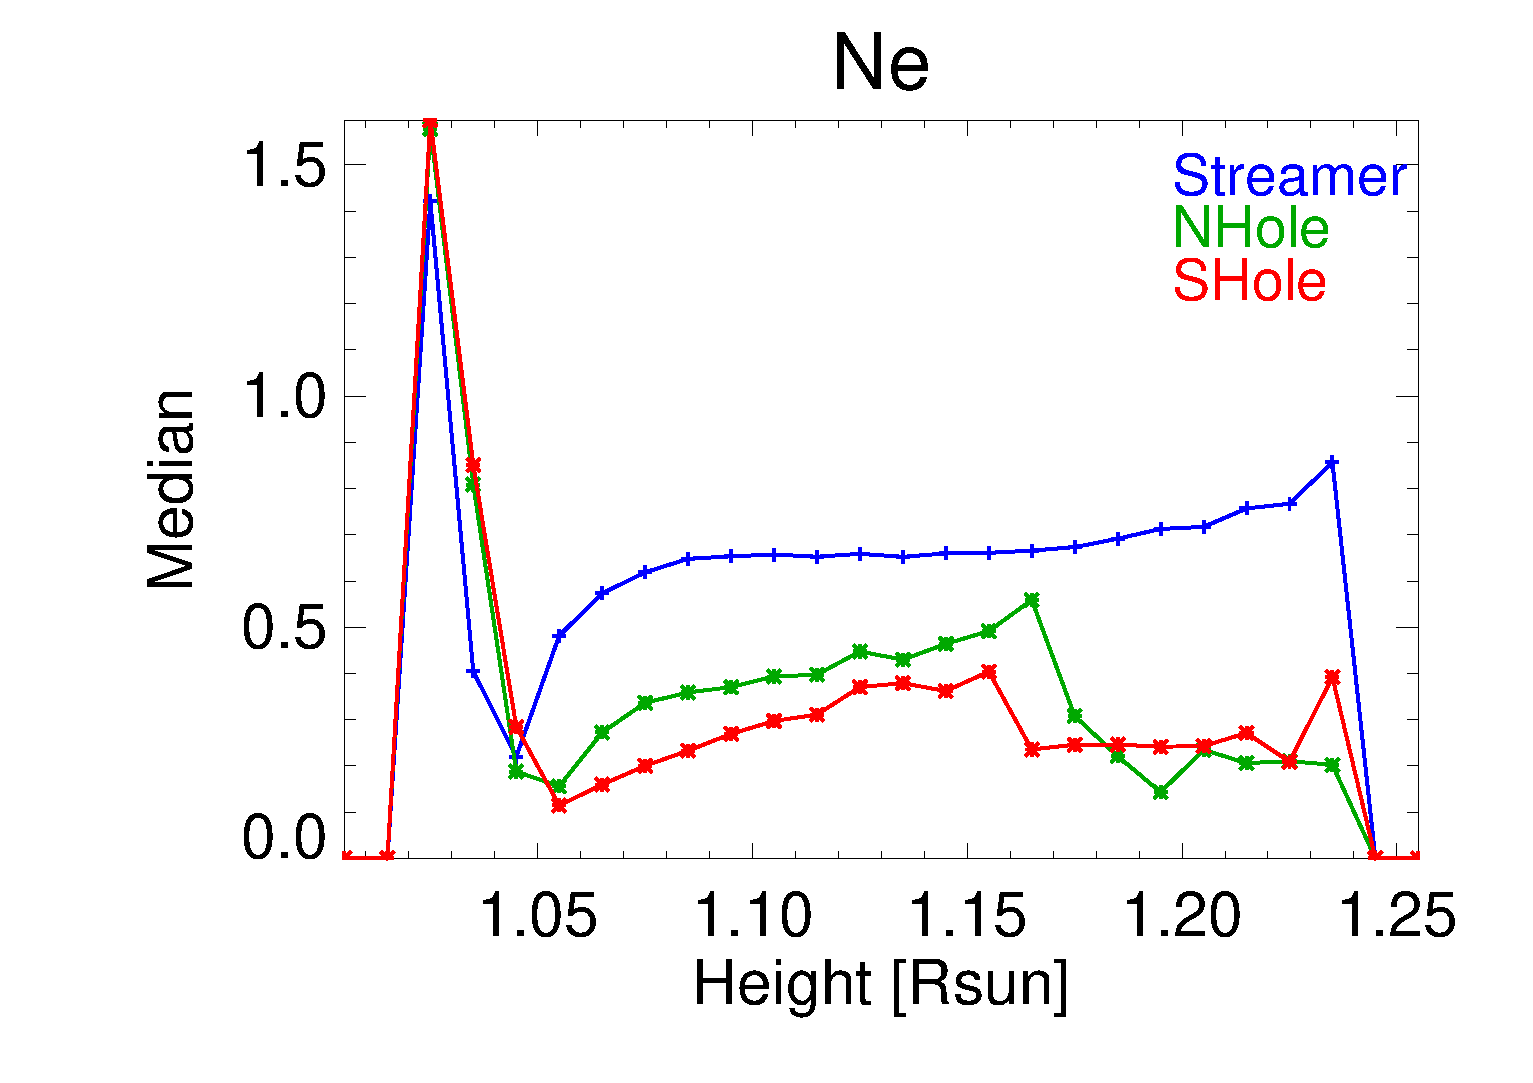
\includegraphics[width=0.45\textwidth]{new_figs/Median_Ne_full_height_run5_disk.eps}
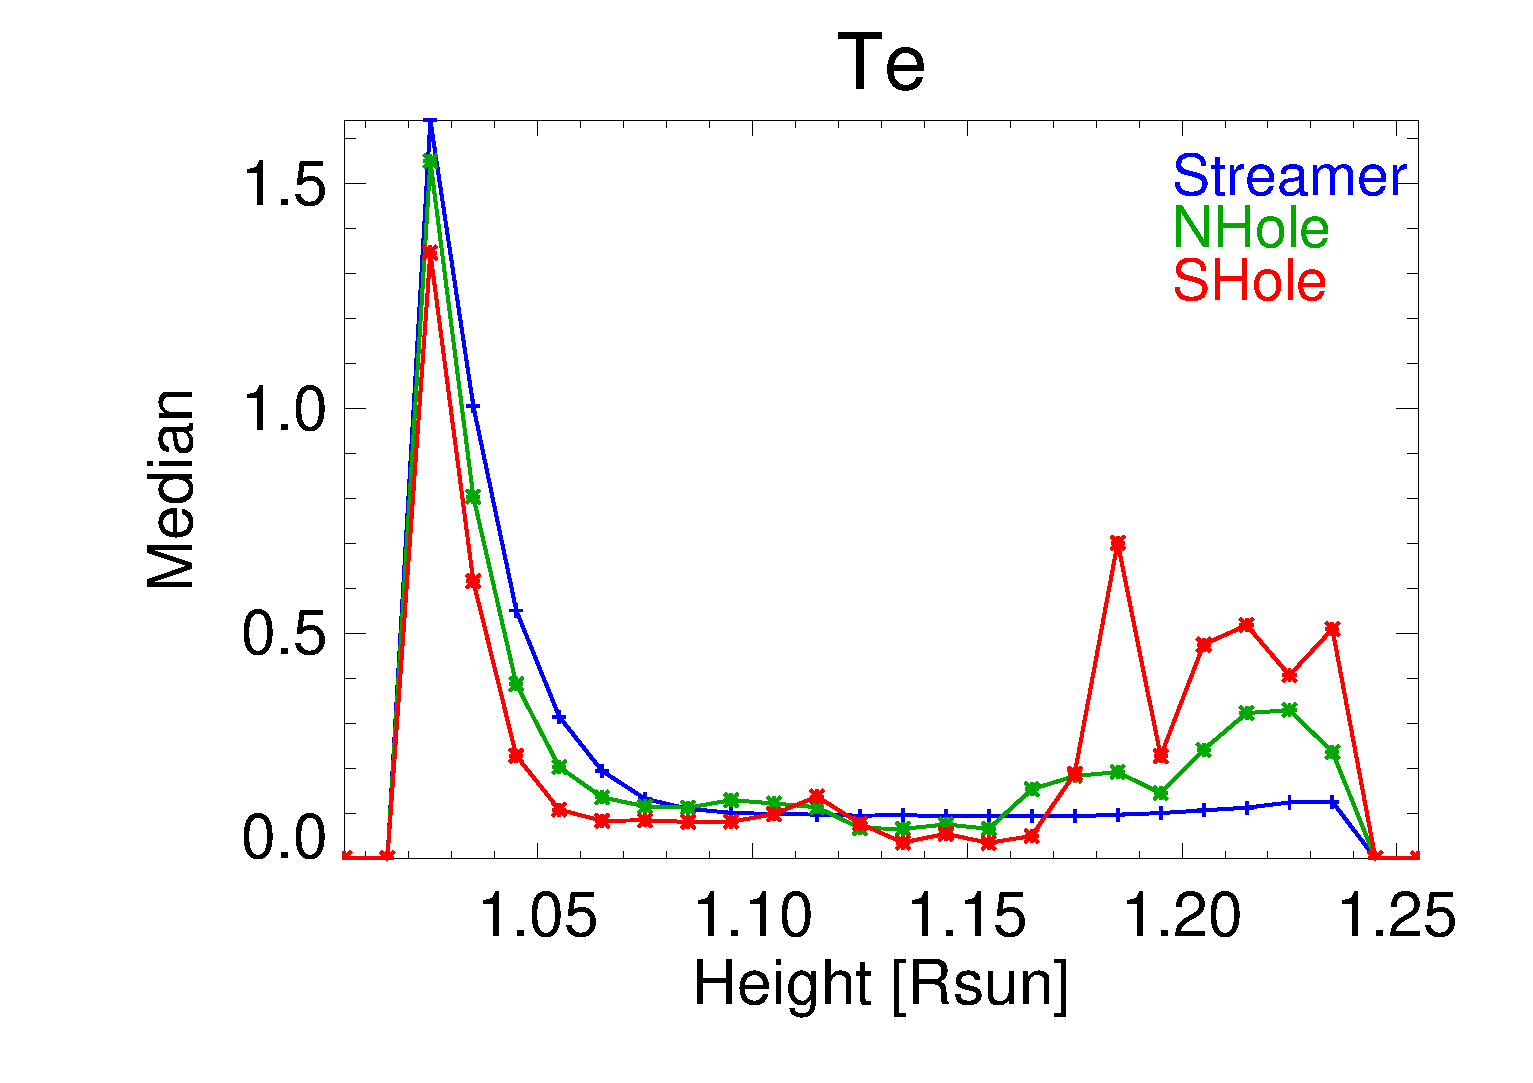
\includegraphics[width=0.45\textwidth]{new_figs/Median_Te_full_height_run5_disk.eps}

\includegraphics[width=0.45\textwidth]{new_figs/2208_magnetograma_adaptivo.png}
\includegraphics[width=0.45\textwidth]{new_figs/CR2081.jpg}
\end{center}
}
%---------------------------------------------------------------------------------------


\frame{ 
\begin{center}
\includegraphics[width=0.75\textwidth]{new_figs/Rpoint-map_5colores_fulleuvi_base.pdf}\\
\includegraphics[width=0.75\textwidth]{new_figs/Rpoint-map_5colores_euvi_base.pdf}
\end{center}
}
%--------------------------------------------------------------------------------















%----------------------------------------------cosas viejas de kcor
\begin{comment}
\frame{
\titulo{Multi-Instrument Tomography (MIT): First Results}
\vspace{-.2cm}
\footnotesize
\begin{center}
%Multi-wavelength Tomography: First Results\\
\includegraphics[height=0.48\textheight]{new_figs/map_ne_kcor.eps}\\ 
\includegraphics[height=0.48\textheight]{new_figs/map_ne_aia.eps}
\end{center}
%\includegraphics[height=0.34\textheight]{new_figs/map_kcor_1205.eps}
%\includegraphics[height=0.34\textheight]{new_figs/map_aia_1205.eps}
}
%--------------------------------------------------
\frame{
\begin{center}
  \azul{Quiet Sun in Streamer Region}\\
\includegraphics[height=0.24\textwidth]{new_figs/Average_Radial_Profiles_KCOR-Tom_vs_DEMT_CR2198_Hh_l45_kcor_subreg-Quiet-region1.eps}
\includegraphics[height=0.24\textwidth]{new_figs/comparison_KCOR-Tom_vs_DEMT_CR2198_Hh_l45_kcor_subreg-Quiet-region1_range1105-1195_Rsun.eps}\\
\azul{Subpolar Open Region}\\
\includegraphics[height=0.24\textwidth]{new_figs/Average_Radial_Profiles_KCOR-Tom_vs_DEMT_CR2198_Hh_l45_kcor_subreg-Open-region_N.eps}
\includegraphics[height=0.24\textwidth]{new_figs/comparison_KCOR-Tom_vs_DEMT_CR2198_Hh_l45_kcor_subreg-Open-region_N_range1105-1155_Rsun.eps}
\end{center}
}
%-----------------------------

%---------------------
\frame{
\titulo{Discussion}
\vspace{-0.5cm}
\begin{itemize}
 \item  $\Eeuv \propto \AvgNE2 = f\,\AvgNe^2$, where \azul{filling factor} is defined as $f\equiv\AvgNE2 / \AvgNe^2$
\salto
\item  $\Ewl \propto \AvgNe$
\salto
\item  Then: $\AvgNe_{\rm{WL}} / \AvgNe_{\rm{EUV}} \propto \sqrt{f}$
\salto
\item  If differences in the results are solely attributed to filling factor:\\
  $f\sim 2$ in subpolar open region, and $f\sim 4$ in quiet sun closed region.
\salto
\item  Note that: $\SigmaNe^2 \equiv \rm{Var}N_e = \AvgNE2 - \AvgNe^2 = \AvgNe^2 \, (f-1)$
\salto
\item  So that: $\SigmaNe / \AvgNe = \sqrt{f-1}$.
\salto
\item  With this interpretation, where $f$ is larger (quiet sun closed region) the electron density probability distribution has larger variance.
\end{itemize}
}

%-----------------------------------------
\frame{
\titulo{Future Work}
%\vspace{-1.cm}
\begin{itemize}
 \item Determination of KCOR-based density error bars (calibration, sky-subtraction).
 \salto
 \item  Other factors can partly explain the observed differences, as [Fe].
\salto	
\item  To refine discrimination of different structures we will next trace results along field lines from MHD models.
\salto
 \item  This work (in progress) is a first step towards future implementation of \azul{Multi-Instrument Tomography (MIT)}. 
\salto
 \item  Future work: MIT aims at using tomographies in WL, EUV and also visible spectral lines (upcoming UCoMP instrument) to simultaneously derive reconstructions for the different physical parameters $\AvgNe, \SigmaNe, f, \rm{[Fe]}$, as well as $\AvgTe, \SigmaTe$. 
 \salto
 \item Perform new comparisons for this and other target rotations.
 
\end{itemize}
\begin{center}
 Thanks a lot for your attention!
\end{center}

}
\end{comment}
\end{document}

% Slides extra
